%\documentclass{beamer}

\documentclass[10pt]{beamer} 
\usetheme[pageofpages=of,% String used between the current page and the
          % total page count.
          alternativetitlepage=true,% Use the fancy title page.
          %titlepagelogo=coca,% Logo for the first page.
          titleline=true
          ]{Torino}
%\usetheme{Frankfurt}
\usecolortheme{chameleon}

\usepackage{graphicx,hyperref,url}
\usepackage[utf8]{inputenc}
\usepackage[T1]{fontenc}
\usepackage[portuges,brazilian]{babel}
%%%\usepackage{wrapfig}
\usepackage{caption}
\usepackage{subfigure}
%\usepackage{subcaption}
\usepackage{latexsym}
\usepackage{amssymb, amsmath}
\usepackage{multicol}
\usepackage{pifont}%,bbding}%%,dingbat} %%% ver manual de simbolos
\usepackage[final]{listings}
\usepackage{comment}


\definecolor{azulclaro}{rgb}{0.9,0.9,0.9}
\definecolor{mygreen}{rgb}{0,0.6,0}
\definecolor{mygray}{rgb}{0.5,0.5,0.5}
\definecolor{mymauve}{rgb}{0.58,0,0.82}
\definecolor{darkgray}{rgb}{.4,.4,.4}
\definecolor{purple}{rgb}{0.65, 0.12, 0.82}

\newcommand{\minizinc}{MiniZinc}

\lstset{ 
  %  label={pgm_ex01},
    backgroundcolor=\color{azulclaro}, 
    language=erlang, %%Miranda,%%Perl,%%%Python, %%Mercury,
    showstringspaces=false,
    basicstyle=\bf\scriptsize\ttfamily,
%%      basicstyle= \footnotesize %%% TESTAR
%%      keywordstyle=\bfseries\color{green!40!black},
    keywordstyle=\textbf{\color{mygreen}}, 
    otherkeywords={*, \%, array, constraint, solve, output,  show, "/\", satisfy, set, of, if, then, elseif, float, search},
%%  keywordstyle=\color{blue},       % keyword style
%%    commentstyle=\itshape\color{purple!40!black},
      commentstyle=\color{orange},    % comment style
      identifierstyle=\color{blue},
      stringstyle=\color{orange},
      stringstyle=\color{mymauve},
      numbers=left,  % where to put the line-numbers; possible values are (none, left, right)
      numbersep=5pt,   % how far the line-numbers are from the code
      numberstyle=\tiny\color{magenta},
      keepspaces=true      
    % %caption={LEGENDA no source PASCAL ficou OK},
}


\graphicspath{{/home/ccs/Dropbox/figs_genericas/}{figuras/}{/home/ccs/Dropbox/CCS/picat}}
\DeclareGraphicsExtensions{.pdf,.png,.jpg}
%Global Background must be put in preamble
%\usebackgroundtemplate{\includegraphics[width=\paperwidth]{amarelinho.pdf}}
%%% \begin{frame}[allowframebreaks=0.8]

% The log drawn in the upper right corner.

%\logo{\centering
%\includegraphics[height=0.050\paperheight]{figuras/logo_SBPO_Peixe.png}
%%\hspace{9.6cm}
%\includegraphics[height=0.027\paperheight]{figuras/logo_udesc_horizontal.jpg}


%%%%%%%%%%%%%%%%%%%%%%%%%%%%%%%%%%%%%%%%%%%%%%%%%%%%%%%%%%%%%%%%%%%%%


\title[Picat]{\fontsize{20}{30}\selectfont \textcolor{black}{PICAT: uma Linguagem Multiparadigma}}

\author[Battisti \& PV]{Claudio Cesar de Sá, Rogério Eduardo da Silva,
    João Herique Faes Battisti, Paulo Victor de Aguiar\\\medskip
    {\small \url{joaobattisti@gmail.com}} \\ 
    {\small \url{pavaguiar@gmail.com}}\\
     {\small \url{claudio.sa@udesc.br}}}

\institute[UDESC]{
    Departamento de Ci\^encia da Computa\c{c}\~ao \\
    Centro de Ci\^encias e Tecnol\'ogias\\
Universidade do Estado de Santa Catarina}

%%%%%%%%%%%%%%%%%%%%%%%%%%%%%%%%%%%%%%%%%%%%%%%%%%%%%%%%%%%%%%%%%%%%%

\begin{document}

\begin{frame}
    \titlepage
\end{frame}

%%%%%%%%%%%%%%%%%%%%%%%%%%%%%%%%%%%%%%%%%%%%%%%%%%%%%%%%%%%%%%%%%%%%%

\begin{frame}[fragile]
\frametitle{Sumário}
\tableofcontents
\end{frame}

\section{Introdução}
\begin{frame}

    \frametitle{Histórico}

    \begin{itemize}
      \item Criada em 2013 por Neng-Fa Zhou e Jonathan Fruhman.

      \item Utilizou o B-Prolog como base de implementação, e ambas utilizam 
      a  programação em lógica baseada na Lógica de Primeira-Ordem (LPO)

      \item Uma evolução ao Prolog após seus mais de 40 anos de sucesso!

      \item Sua atual versão é a 2.0 (\today)

    \end{itemize}
\end{frame}

%%%%%%%%%%%%%%%%%%%%%%%%%%%%%%%%%%%%%%%%%%%%%%%%%%%%%%%%%%%%%%%%%%%%%

%\section{Isso é outra seção}
\begin{frame}
    \frametitle{Picat é Multiparadigma:}
    \begin{itemize}
      \item Imperativo -- Procedural
      \item Funcional
      \item \underline{Lógico}
    %  \item 
    \end{itemize}
\end{frame}

%%%%%%%%%%%%%%%%%%%%%%%%%%%%%%%%%%%%%%%%%%%%%%%%%%%%%%%%%%%%%%%%%%%%%

\begin{frame}
    \frametitle{Algumas Características:}

    \begin{itemize}
      \item Sintaxe $\Rightarrow $ elegância do código
      \item Velocidade de execução
      \item Portabilidade (todas plataformas)
      \item Extensão há outras ferramentas
      
    \end{itemize}
\end{frame}

%%%%%%%%%%%%%%%%%%%%%%%%%%%%%%%%%%%%%%%%%%%%%%%%%%%%%%%%%%%%%%%%%%%%%

\begin{frame}
    \frametitle{Algumas Características:}
    \begin{itemize}
      \item Terminologia: segue as bases teóricas da linguagem Prolog.
    
      \item Na \textbf{l}ógica de \textbf{p}rimeira-\textbf{o}rdem (LPO) os objetos são chamados por \textbf{termos}.
      
      \item O destaque de Picat é a sua natureza declarativa, funcional, tipagem dinâmica, e sintaxe \textit{açucarada}
      
      \item \texttt{PICAT} é um anacrônico onde cada letra representa uma característica  de sua funcionalidade (operacionalidade).
    
    \end{itemize}
\end{frame}

%%%%%%%%%%%%%%%%%%%%%%%%%%%%%%%%%%%%%%%%%%%%%%%%%%%%%%%%%%%%%%%%%%%%%

\section{Características}
\begin{frame}
    \frametitle{Anacrônico: \textbf{P.I.C.A.T.}}
 
 
 \begin{description}
   
 
 \item [P:] \textit{Pattern-matching}:  Utiliza o conceito de casamento padrão da LPO
 
 \item [I:]  \textit{Intuitive}: oferece atribuições e laços de repetições análogo as outras linguagens de programação
 
  \item [C:]   \textit{Constraints}: suporta a programação por restrições
 
     \item [A:] \textit{Actors}: suporte as chamadas a eventos, os atores (futuro gráfico) 
 
  \item [T:] \textit{Tabling}: implementa a técnica de \textit{memoization}, com soluções imediatas para problemas de Programação Dinâmica.
   
  
\end{description}
\end{frame}

%%%%%%%%%%%%%%%%%%%%%%%%%%%%%%%%%%%%%%%%%%%%%%%%%%%%%%%%%%%%%%%%%%%%%

\begin{frame}
    
\end{frame}

%%%%%%%%%%%%%%%%%%%%%%%%%%%%%%%%%%%%%%%%%%%%%%%%%%%%%%%%%%%%%%%%%%%%%

\begin{frame}
    \end{frame}

%%%%%%%%%%%%%%%%%%%%%%%%%%%%%%%%%%%%%%%%%%%%%%%%%%%%%%%%%%%%%%%%%%%%%

%%%%%%%%%%%%%%%%%%%%%%%%%%%%%%%%%%%%%%%%%%%%%%%%%%%%%%%%%%%%%%%%%%%%%

\begin{frame}
    \frametitle{Instalação do PICAT}

     Tenham um editor de código de programa.\\
     Sugestão: \textit{geany} ou \textit{sublime}



\end{frame}

%%%%%%%%%%%%%%%%%%%%%%%%%%%%%%%%%%%%%%%%%%%%%%%%%%%%%%%%%%%%%%%%%%%%%


%%%%%%%%%%%%%%%%%%%%%%%%%%%%%%%%%%%%%%%%%%%%%%%%%%%%%%%%%%%%%%%%%%%%%

\begin{frame}
    \frametitle{Sistema de Programação}
    \begin{itemize}
     \item Picat é uma linguagem de multiplataforma, disponível em qualquer arquitetura de processamento e também de sistema operacional
     \item Utiliza a extensão .pi em seus arquivos de código fonte. 
     \item Existem 2 modos de utilização do Picat: Modo linha de comando e Modo Interativo. 
    \end{itemize}
\end{frame}

%%%%%%%%%%%%%%%%%%%%%%%%%%%%%%%%%%%%%%%%%%%%%%%%%%%%%%%%%%%%%%%%%%%%%


%%%%%%%%%%%%%%%%%%%%%%%%%%%%%%%%%%%%%%%%%%%%%%%%%%%%%%%%%%%%%%%%%%%%%

\section{Tipos de Dados}

\begin{frame}
\frametitle{Tipos de Dados}
\begin{figure}[!ht]
\centering
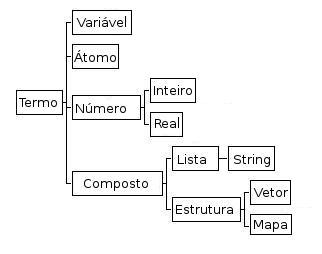
\includegraphics[width=.6\textwidth]{figures/tipos_dados_picat_traduzido.jpg}
\caption{Hierarquia dos Tipos de dados}
\label{Hiera}
\end{figure}
\end{frame}

%%%%%%%%%%%%%%%%%%%%%%%%%%%%%%%%%%%%%%%%%%%%%%%%%%%%%%%%%%%%%%%%%%%%%

%%%%%%%%%%%%%%%%%%%%%%%%%%%%%%%%%%%%%%%%%%%%%%%%%%%%%%%%%%%%%%%%%%%%%

\begin{frame}
    \frametitle{Número}
    \texttt{Picat> A = 5, B = 7, number(A), number(B),
    max(A, B) = Maximo, min(A, B) = Minimo.}\\
  
    \texttt{A = 5}\\
    \texttt{B = 7}\\
    \texttt{Maximo = 7}\\
    \texttt{Minimo = 5}\\
    \texttt{yes.}
\end{frame}

%%%%%%%%%%%%%%%%%%%%%%%%%%%%%%%%%%%%%%%%%%%%%%%%%%%%%%%%%%%%%%%%%%%%%


%%%%%%%%%%%%%%%%%%%%%%%%%%%%%%%%%%%%%%%%%%%%%%%%%%%%%%%%%%%%%%%%%%%%%

\section{Exemplos}
\begin{frame}
    \frametitle{Exemplos}
    \begin{figure}[!ht]
    \centering
    
\includegraphics[width=.6\textwidth]{figures/exercicio.jpg}
    %\caption{Hierarquia dos Tipos de dados}
    %\label{Hiera}
    \end{figure}
\end{frame}

%%%%%%%%%%%%%%%%%%%%%%%%%%%%%%%%%%%%%%%%%%%%%%%%%%%%%%%%%%%%%%%%%%%%%

\begin{frame}
    \frametitle{Atribuição}
     \texttt{Picat> X := 7, X := X + 7, X := X + 7.}\\
     \texttt{X = 21}
\end{frame}

%%%%%%%%%%%%%%%%%%%%%%%%%%%%%%%%%%%%%%%%%%%%%%%%%%%%%%%%%%%%%%%%%%%%%

\begin{frame}
    \frametitle{Estruturas de Controle}
     \texttt{ex1 =>}\\
     \texttt{X:=3, Y:=4,}\\
     \texttt{if(X >= Y)}\\
     \texttt{then printf("\%d", X)}\\
     \texttt{else printf("\%d", Y)}\\
     \texttt{end.}
\end{frame}

%%%%%%%%%%%%%%%%%%%%%%%%%%%%%%%%%%%%%%%%%%%%%%%%%%%%%%%%%%%%%%%%%%%%%

%%%%%%%%%%%%%%%%%%%%%%%%%%%%%%%%%%%%%%%%%%%%%%%%%%%%%%%%%%%%%%%%%%%%%
\subsection{Entradas e Sa\'idas}
\begin{frame}
    \frametitle{Entradas e Saídas}
    \texttt{main =>}\\
    \texttt{printf("Digite dois números: "),}\\
    \texttt{N$\_real01 = read\_$real(),}\\
    \texttt{N$\_real02 = read\_$real(),}\\
    \texttt{Media = (N$\_real01+N\_real$02)/2,}\\
    \texttt{printf("A média é: \%6.2f", Media),}\\
    \texttt{printf("$\backslash n ......FIM....... \backslash$ n").}
\end{frame}

%%%%%%%%%%%%%%%%%%%%%%%%%%%%%%%%%%%%%%%%%%%%%%%%%%%%%%%%%%%%%%%%%%%%%

%%%%%%%%%%%%%%%%%%%%%%%%%%%%%%%%%%%%%%%%%%%%%%%%%%%%%%%%%%%%%%%%%%%%%

%%%%%%%%%%%%%%%%%%%%%%%%%%%%%%%%%%%%%%%%%%%%%%%%%%%%%%%%%%%%%%%%%%%%%

\begin{frame}
    \frametitle{Regras  em Lógica -- os pais!}
    \begin{itemize}
    
    \item $pai(platao, luna)$ \hspace{1.5cm} leia-se: \textit{Platão é o pai de Luna}
    \item $pai(platao, péricles)$ \hspace{1.5cm} leia-se: \textit{Platão é o pai de Péricles}
    \item $pai(epimenides, platao)$ \hspace{1.5cm} leia-se: \textit{Sócrates é o pai de Platão}
    
    \pause
    
    \item Alguém que é avô tem um filho que é um pai de alguém
    \pause
    
    \item Alguém que é irmão tem o mesmo pai e não é irmão consigo mesmo
    \pause
    
    \item \textcolor{red}{As regras estão nos slides de lógica}

    \item  $\Rightarrow $ as saídas são \textbf{particularizações} (PU e PE)
 
    \end{itemize}
\end{frame}

\begin{frame}[allowframebreaks=0.9]
 \frametitle{Regras em PICAT}

\lstinputlisting{../regras_ex_02.pi}

\end{frame}

%%%%%%%%%%%%%%%%%%%%%%%%%%%%%%%%%%%%%%%%%%%%%%%%%%%%%%%%%%%%%%%%%%%%%
%%%%%%%%%%%%%%%%%%%%%%%%%%%%%%%%%%%%%%%%%%%%%%%%%%%%%%%%%%%%%%%%%

\section{Conclusão}
\begin{frame}
    \frametitle{Conclusão}
    \begin{itemize}
    \item PICAT é uma linguagem nova (2013), desconhecida, revolucionária e com um futuro promissor para áreas de pesquisas e utilização comercial.
    \item Atualmente há pouco material disponível e uma comunidade pequena de usuários
    \item Uso acadêmico
    \item
    \end{itemize}
\end{frame}

%%%%%%%%%%%%%%%%%%%%%%%%%%%%%%%%%%%%%%%%%%%%%%%%%%%%%%%%%%%%%%%%%%%%%

%\section{Referências}
\begin{frame}
    \frametitle{Referências}
    \begin{itemize}
    \item O User Guide que está no diretório  doc/
     \item \url{https://github.com/claudiosa/CCS/tree/master/picat}
     \item \url{http://picat-lang.org/}
    \item Assinem o fórum do PICAT

    \item Site do Hakan  Kjellerstrand 
    \item Site do Román Bartak
    \item Site do Dymichenko
    
    \end{itemize}
\end{frame}

%%%%%%%%%%%%%%%%%%%%%%%%%%%%%%%%%%%%%%%%%%%%%%%%%%%%%%%%%%%%%%%%%%%%%

%\section{Questionário}
\begin{frame}
    \frametitle{Obrigado}

 Retornem os comentários para .........


\end{frame}

\end{document}
